\begin{frame}{Introduction}
  Systèmes d'indexation :
  \begin{itemize}
    \item Solr 
      \begin{itemize}
        \item Open Source
        \item Fondation Apache
      \end{itemize}
    \item Sphinx
    \item ElasticSearch
  \end{itemize}
  \medskip \caveat{Dans ce qui suit nous allons parler des {\bf documents Solr}
  pour désigner la liste des champs transmise à l'index, et les distinguer des
  {\bf documents applicatifs} de notre base de données documentaire}
      
\caveat{Solr peut  être vu comme une base de données spécialisée dans la
recherche d'information: on y insère des documents (Solr), conformes à un
schéma, et on peut rechercher des documents (Solr). }

\end{frame}

\begin{frame}{À quoi sert Solr ?}
  \begin{itemize}
    \item Solr est une application spécialisée dans la recherche
    \item Repose sur l'index Lucene (Apache, auparavant projet distinct)
      \medskip
    \item Efficacité très élevée pour la recherche
    \item Moins pour les autres tâches de base de données (stockage, mise à jour
      fréquentes)
    \item Souvent c'est donc un {\bf complément} d'un serveur de BDD
      (relationnelle ou documentaire)
    \item Spécialisé dans les recherches non structurées
        \item ex. : recherche par mot-clef dans un site Web
          \begin{itemize}
            \item Documents gérés par MySQL
            \item Extraction des textes et construction de l'index avec Solr
            \item Le champ ``Recherche'' interroge Solr, qui répond
          \end{itemize}
  \end{itemize}
\end{frame} % ending frame Résumé: à quoi sert Solr ?

 \begin{frame}{Architecture d'une application avec moteur de recherche}
   \begin{center}
     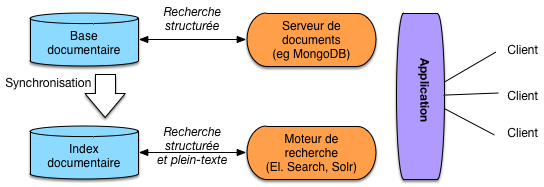
\includegraphics[width=11cm]{../figures/archi-ri.png}
   \end{center}
 \end{frame} % ending frame Architecture d'une application avec moteur de recherche

%La figure :ref:`archi-ri` montre une architecture typique, en prenant pour
%exemple une base de données MongoDB. Les *documents (applicatifs)* sont donc
%dans la base MongoDB qui fournit des fonctionnalités de recherche structurées.
%On peut indexer la collection des documents applicatifs en extrayant des
%"champs" formant dans *documents (Solr)*, fournis à l'index qui se charge de les
%organiser pour satisfaire efficacement des requêtes (nous verrons comment).
%L'application peut alors soit s'adresser au serveur MongoDB, soit au serveur
%Solr.

%Un scénario typique est celui d'une recherche par mot-clé dans un site. Les données
%du site sont probablement gérées classiquement par, disons, MySQL. On extrait 
%de la base MySQL tous les textes à indexer et on en fait des documents Solr 
%que l'on confie à Solr. Ce dernier se charge alors de réponde à la fonctionnalité ``Search``
%que l'on trouve couramment sur tous les types de site.

%%Nous allons commencer notre découverte des systèmes d'indexation avec le moteur de recherche 
%%`Solr <http://lucene.apache.org/solr>`_,
%%un des  outils Open Source les plus répandus (avec Sphinx et ElasticSearch, que
%%nous examinerons ultérieurement pour la simplicité de son modèle de passage
%%à l'échelle par distribution).  Solr est une application construite sur
%%les index du système Lucene. Pour l'instant nous allons installer Solr,
%%indexer nos collections et les interroger. Dans un second temps nous
%%regarderons en interne comment fonctionne le système.

\begin{frame}[fragile]{Installation}

  Installation très simple
  \begin{itemize}
    \item pré requis : Java 1.7 (au moins)
      \smallskip
    \item télécharger l'archive de la dernière version stable (4.10.2) :\\
\url{http://lucene.apache.org/solr/downloads.html}
\item la décompresser quelque part (``soldir'') :\\
\begin{minted}[frame=lines,
               baselinestretch=.9,
               fontsize=\footnotesize,
               framesep=2mm]{bash}
  tar -xvzf solr-4.10.2.tgz ~/soldir
\end{minted}
  \end{itemize}
  \medskip
  Démarrage 
\begin{itemize}
    \item aller dans ~/soldir/example :\\
\begin{minted}[ baselinestretch=.9,
               fontsize=\footnotesize,
               framesep=2mm]{bash}
      cd ~/soldir/example
\end{minted}
    \item taper la commande suivante :\\
\begin{minted}[ baselinestretch=.9,
               fontsize=\footnotesize,
               framesep=2mm]{bash}
      java -jar start.jar
\end{minted}
    \item laisser ce terminal ouvert
    \item lancer un navigateur et aller à l'adresse :\\
\begin{minted}[ baselinestretch=.9,
               fontsize=\footnotesize,
               framesep=2mm]{bash}
  http://localhost:8983/solr
\end{minted}

  \end{itemize}
\end{frame}

   \begin{frame}{Admin}
     \begin{center}
       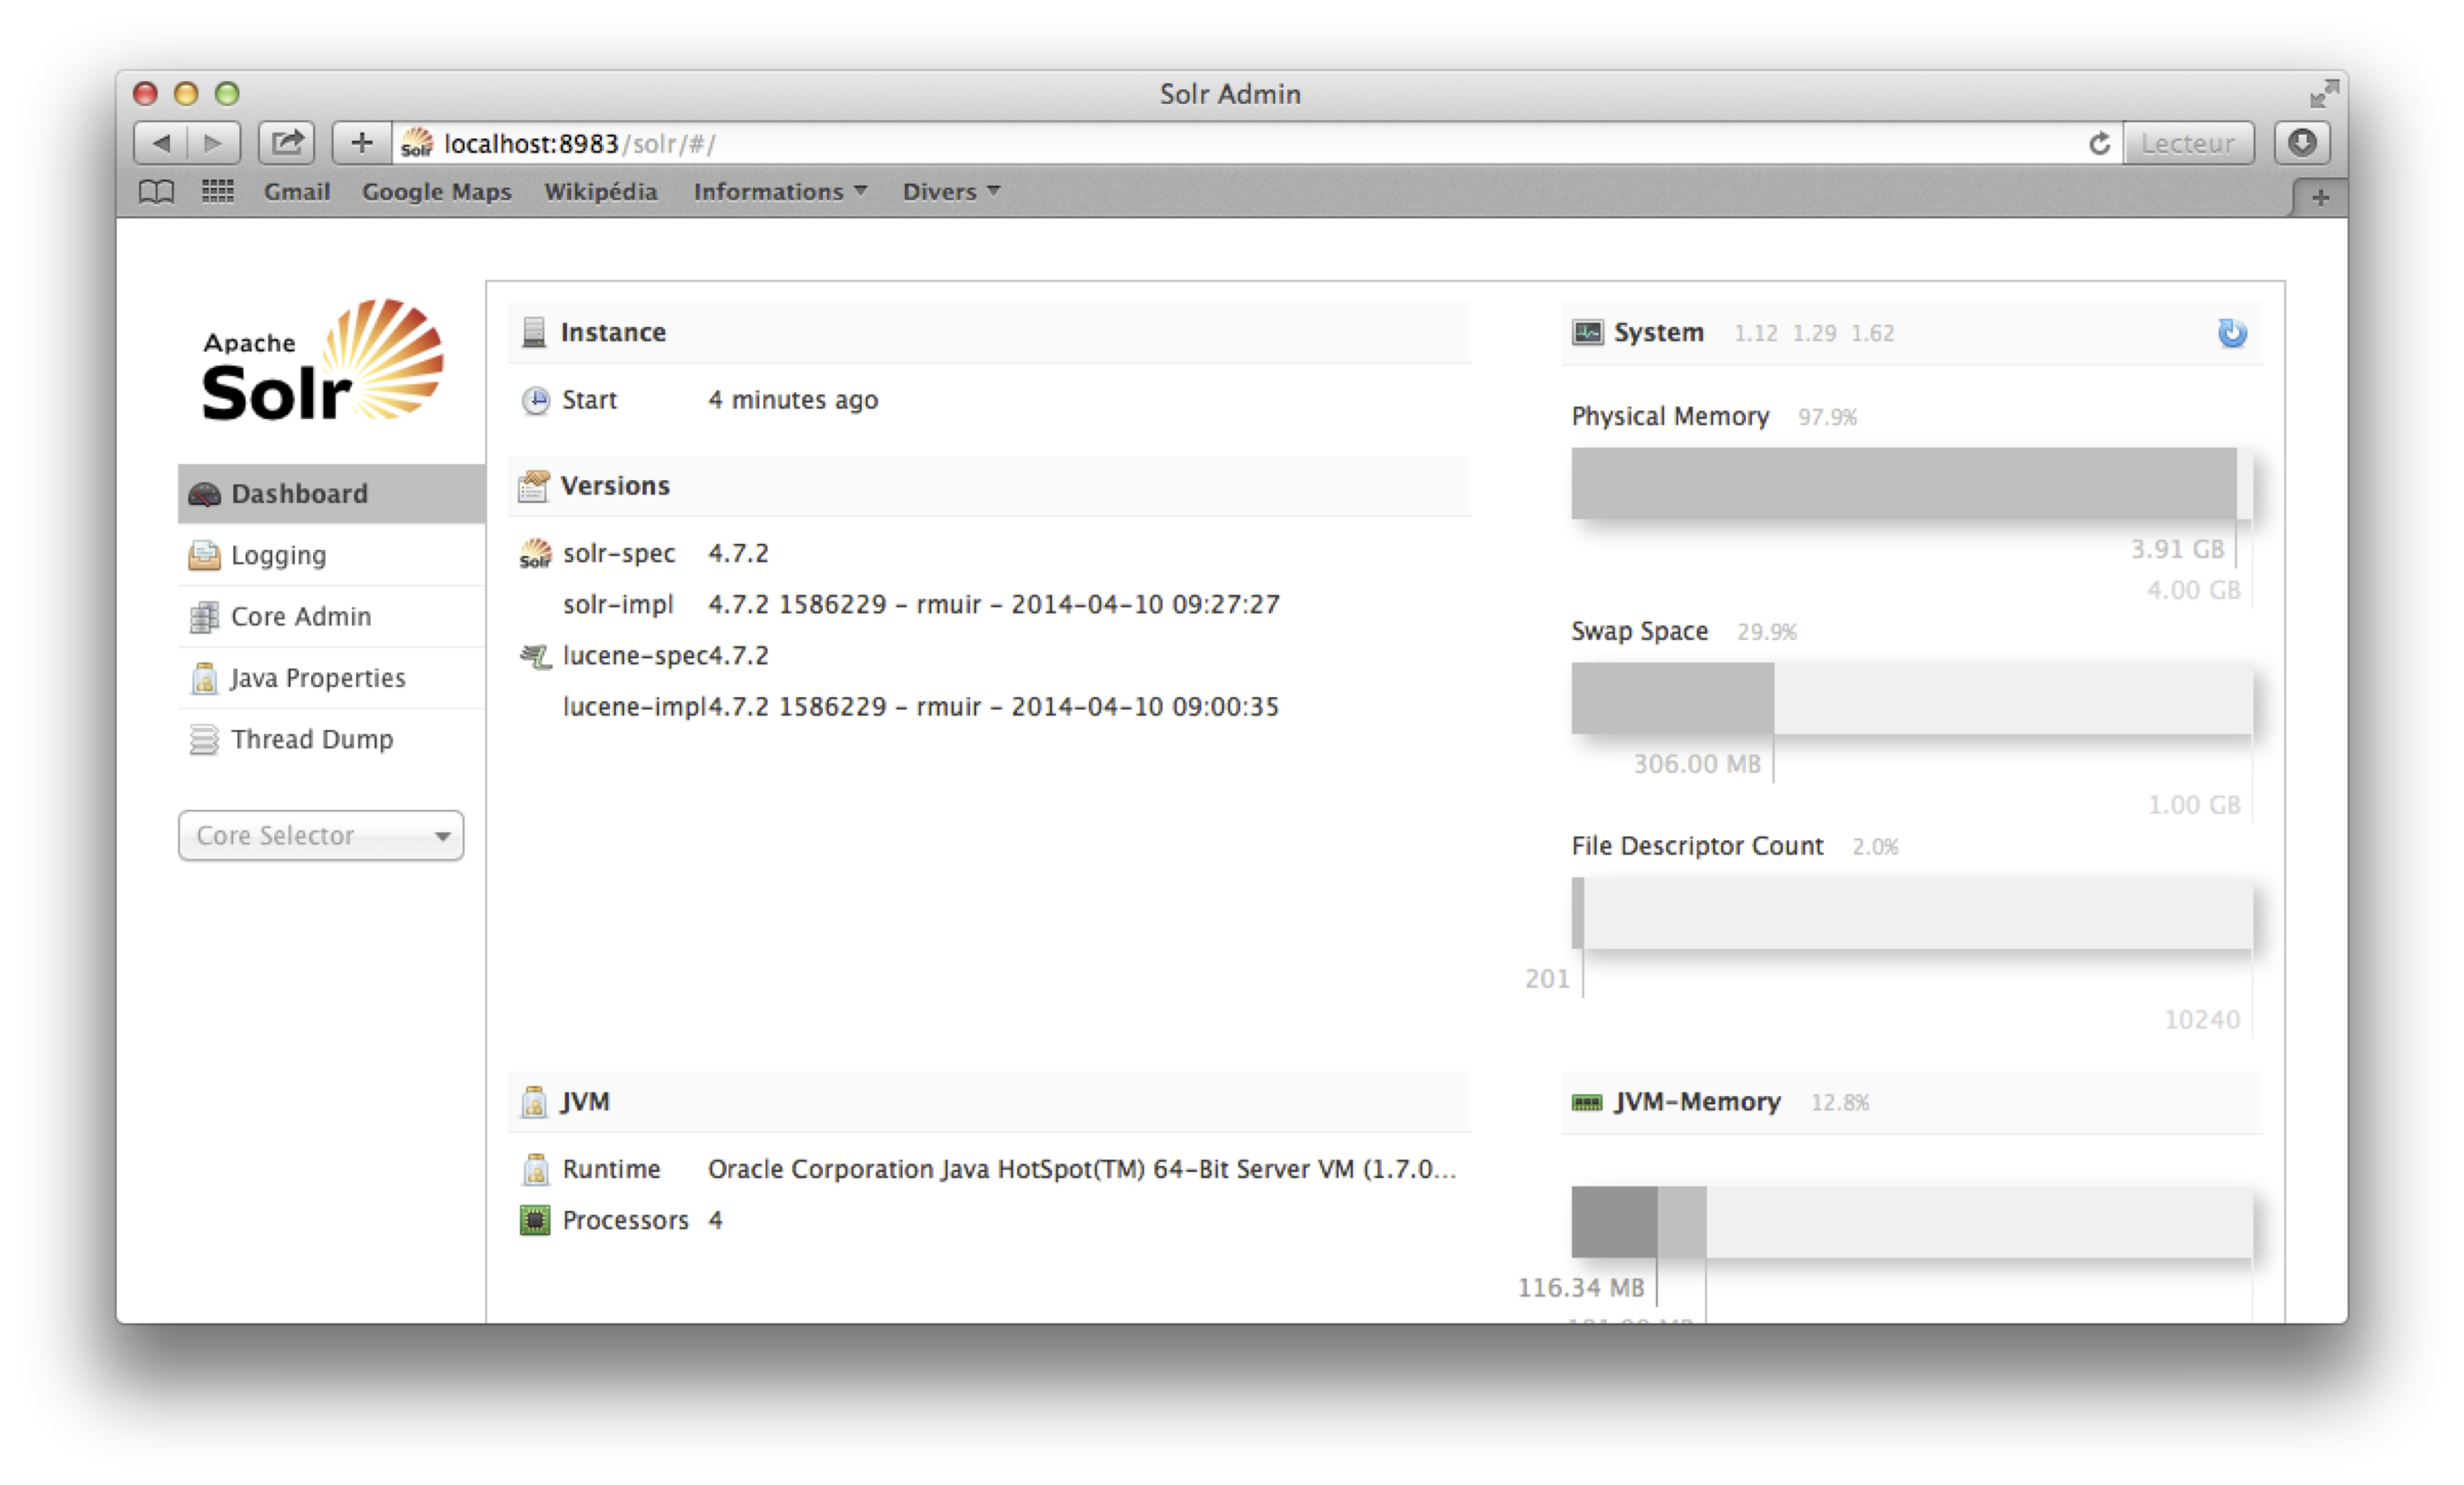
\includegraphics[width=11cm]{../figures/solr-admin.png}
     \end{center}
   \end{frame} % ending frame Admin

      
\begin{frame}[fragile]{Insertion de documents}

   \begin{itemize}
     \item Solr fournit des services REST (HTTP) pour recevoir/envoyer des
       instructions
     \item codées en JSON ou XML
\item insérer de documents
\item effectuer des requêtes
\smallskip
\item accessible à l'URL \url{http://localhost:8983/solr/update}
   \end{itemize}
Exemple pour une indexation:
\begin{itemize}
  \item attente de document de type ``Content-type:application/xml`` (binaire)
  \item on utilise curl :\\
curl http://localhost:8983/solr/update --data-binary @item.xml  -H 'Content-type:application/xml'
\end{itemize}
\end{frame}
   
\begin{frame}{Indexation en pratique}
     \begin{itemize}
       \item dans le dossier ``soldir/example/exampledocs/'', il y a par
         exemple :\\
         solr.xml
       \item on peut utiliser curl, mais aussi deux utilitaires fournis par
         Solr:
         \begin{itemize}
           \item post.jar :\\
             java -jar post.jar solr.xml
           \item post.sh :\\
             ./post.sh *.xml
         \end{itemize}
   \item sélectionner ensuite le core ``Collection1'' dans la barre de
     navigation
     \end{itemize}
\end{frame}

   
%Vous devriez obtenir une confirmation de l'insertion (c'est plus clair avec le
%programme java). Reportez-vous maintenant à l'interface Web, et sélectionnez le
%*core* ``Collection1`` dans la barre de navigation gauche. Vous devriez obtenir
%l'affichage de la figure :ref:`solr-apres-insert`, et la confirmation que des
%documents ont été indexés.
       
\begin{frame}{Consultation de la Collection1}
  \begin{center}
    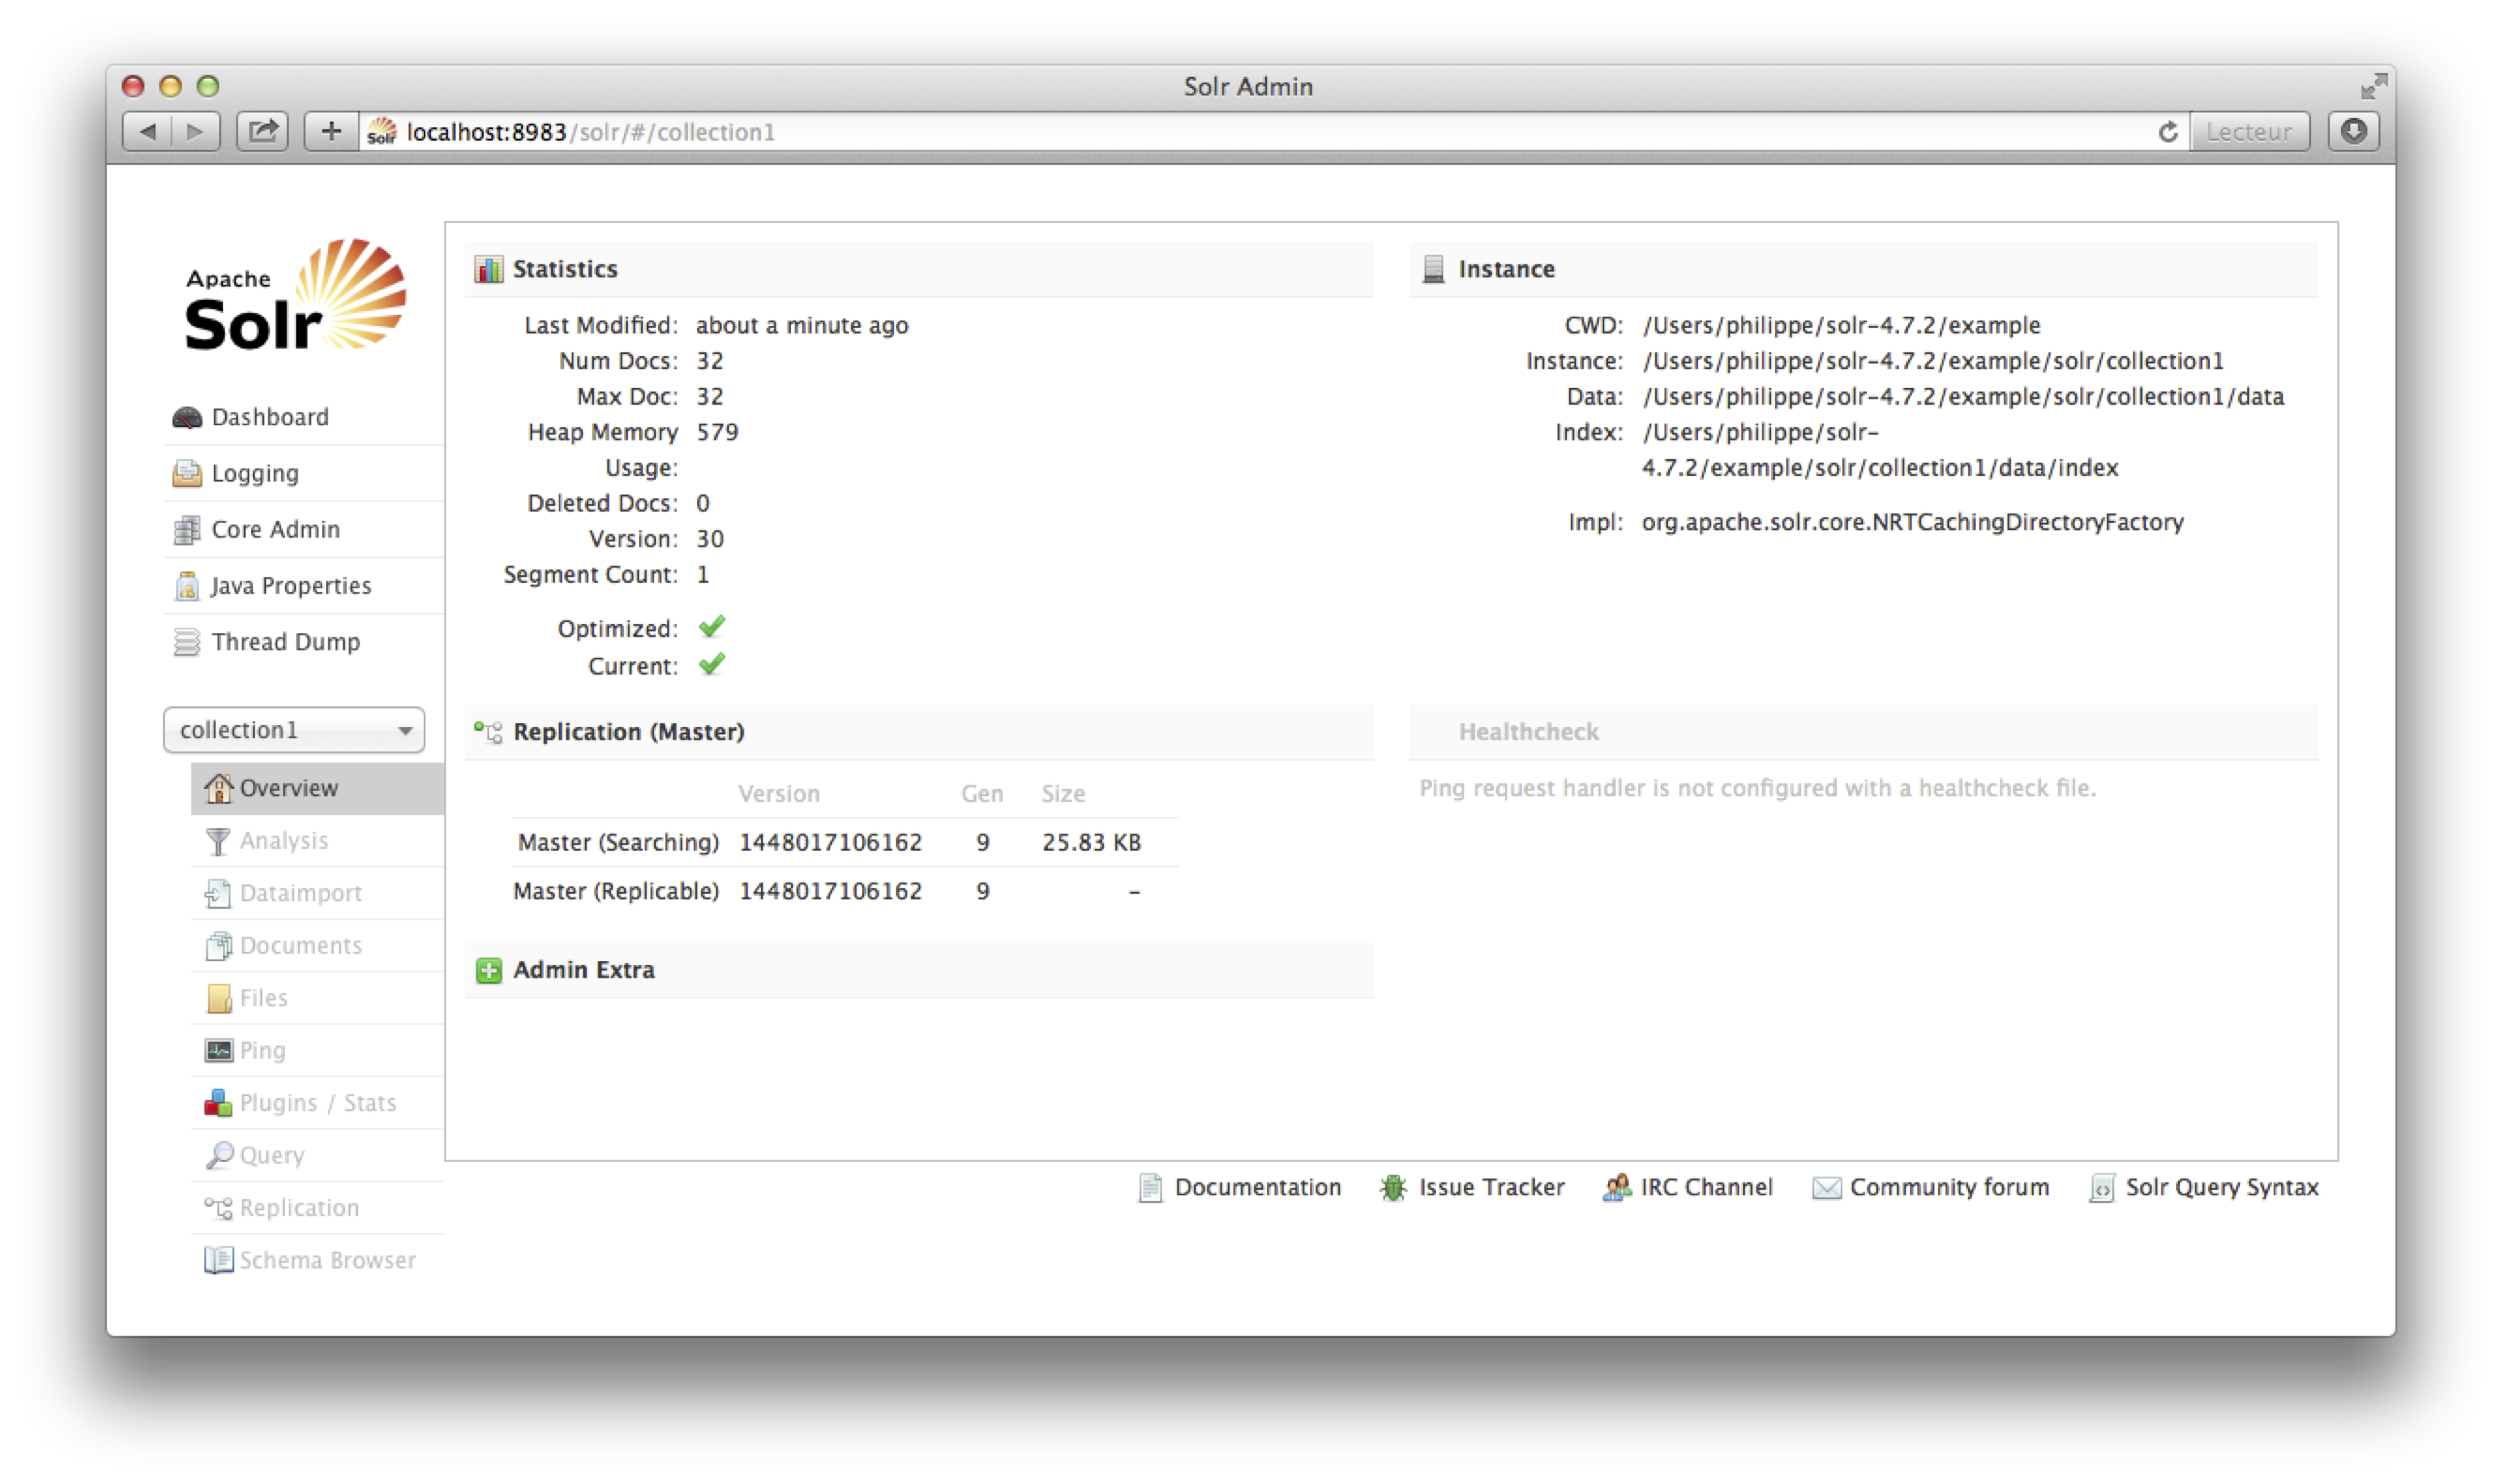
\includegraphics[width=11cm]{../figures/solr-apres-insert.png}
  \end{center}
\end{frame} % ending frame frametitle




\begin{frame}[fragile]{Contenus des documents indexés}
\begin{minted}[frame=lines,
               baselinestretch=.9,
               fontsize=\footnotesize,
               framesep=2mm]{xml}
<add>
 <doc>
  <field name="id">SOLR1000</field>
  <field name="name">Solr, the Enterprise Search Server</field>
  <field name="manu">Apache Software Foundation</field>
  <field name="cat">software</field>
  <field name="cat">search</field>
  <field name="features">Advanced Full-Text Search Capabilities using Lucene</field>
  <field name="features">Optimized for High Volume Web Traffic</field>
  <field name="price">0</field>
  <field name="popularity">10</field>
  <field name="inStock">true</field>
  <field name="incubationdate_dt">2006-01-17T00:00:00.000Z</field>
 </doc>
</add>
\end{minted}
\smallskip
\begin{itemize}
\item Le document est constitué de {\bf champs} ({\bf fields}), 
%\item chaque champ est indexé séparément
\item le nom du champ est indiqué par l'attribut \variable{name}. 
\item il faut qu'ils aient été déclarés au préalable dans le {\bf schéma} de l'index.
  \begin{itemize}
    \item \variable{price} est déclaré comme numérique
    \item \variable{features} comme chaîne de caractères
  \end{itemize}
\end{itemize}
\end{frame}

   %%\begin{frame}[fragile]{Exemple de XML et de JSON}
%%\begin{minted}[linenos,
               %%frame=lines,
               %%baselinestretch=.9,
               %%fontsize=\footnotesize,
               %%framesep=2mm]{json}
%%{
    %%"menu": {
        %%"id": "file",
        %%"value": "File",
        %%"popup": {
            %%"menuitem": [
                %%{ "value": "New", "onclick": "CreateNewDoc()" },
                %%{ "value": "Open", "onclick": "OpenDoc()" },
                %%{ "value": "Close", "onclick": "CloseDoc()" }
            %%]
        %%}
    %%}
%%}
%%\end{minted}
%%\begin{minted}[linenos,
               %%frame=lines,
               %%baselinestretch=.9,
               %%fontsize=\footnotesize,
               %%framesep=2mm]{json}
%%<menu id="file" value="File">
 %%<popup>
   %%<menuitem value="New" onclick="CreateNewDoc()" />
   %%<menuitem value="Open" onclick="OpenDoc()" />
   %%<menuitem value="Close" onclick="CloseDoc()" />
 %%</popup>
%%</menu>
%%\end{minted}
   %%\end{frame}

   %%\subsection{Interroger un index}

\begin{frame}[fragile]{Interroger un index avec Solr}
  \begin{itemize}
    \item Solr dispose d'une interface REST pour {\bf rechercher} des documents :\\
\begin{minted}[frame=lines,
               baselinestretch=.9,
               fontsize=\footnotesize,
               framesep=2mm]{text}
      http://localhost:8983/solr/select?q=video
\end{minted}
  \item dans le navigateur, ou avec curl :\\
\begin{minted}[frame=lines,
               baselinestretch=.9,
               fontsize=\footnotesize,
               framesep=2mm]{text}
    curl http://localhost:8983/solr/select?q=video
\end{minted}
\item La réponse est formattée en XML. On peut aussi demander un retour en JSON :\\
\begin{minted}[frame=lines,
               baselinestretch=.9,
               fontsize=\footnotesize,
               framesep=2mm]{text}
    http://localhost:8983/solr/select?q=video&wt=json&indent=yes
\end{minted}
  \item interface d'administration intégrée
  \end{itemize}
\end{frame}

\begin{frame}{Fenêtre d'interrogation de Solr}
  \begin{center}
    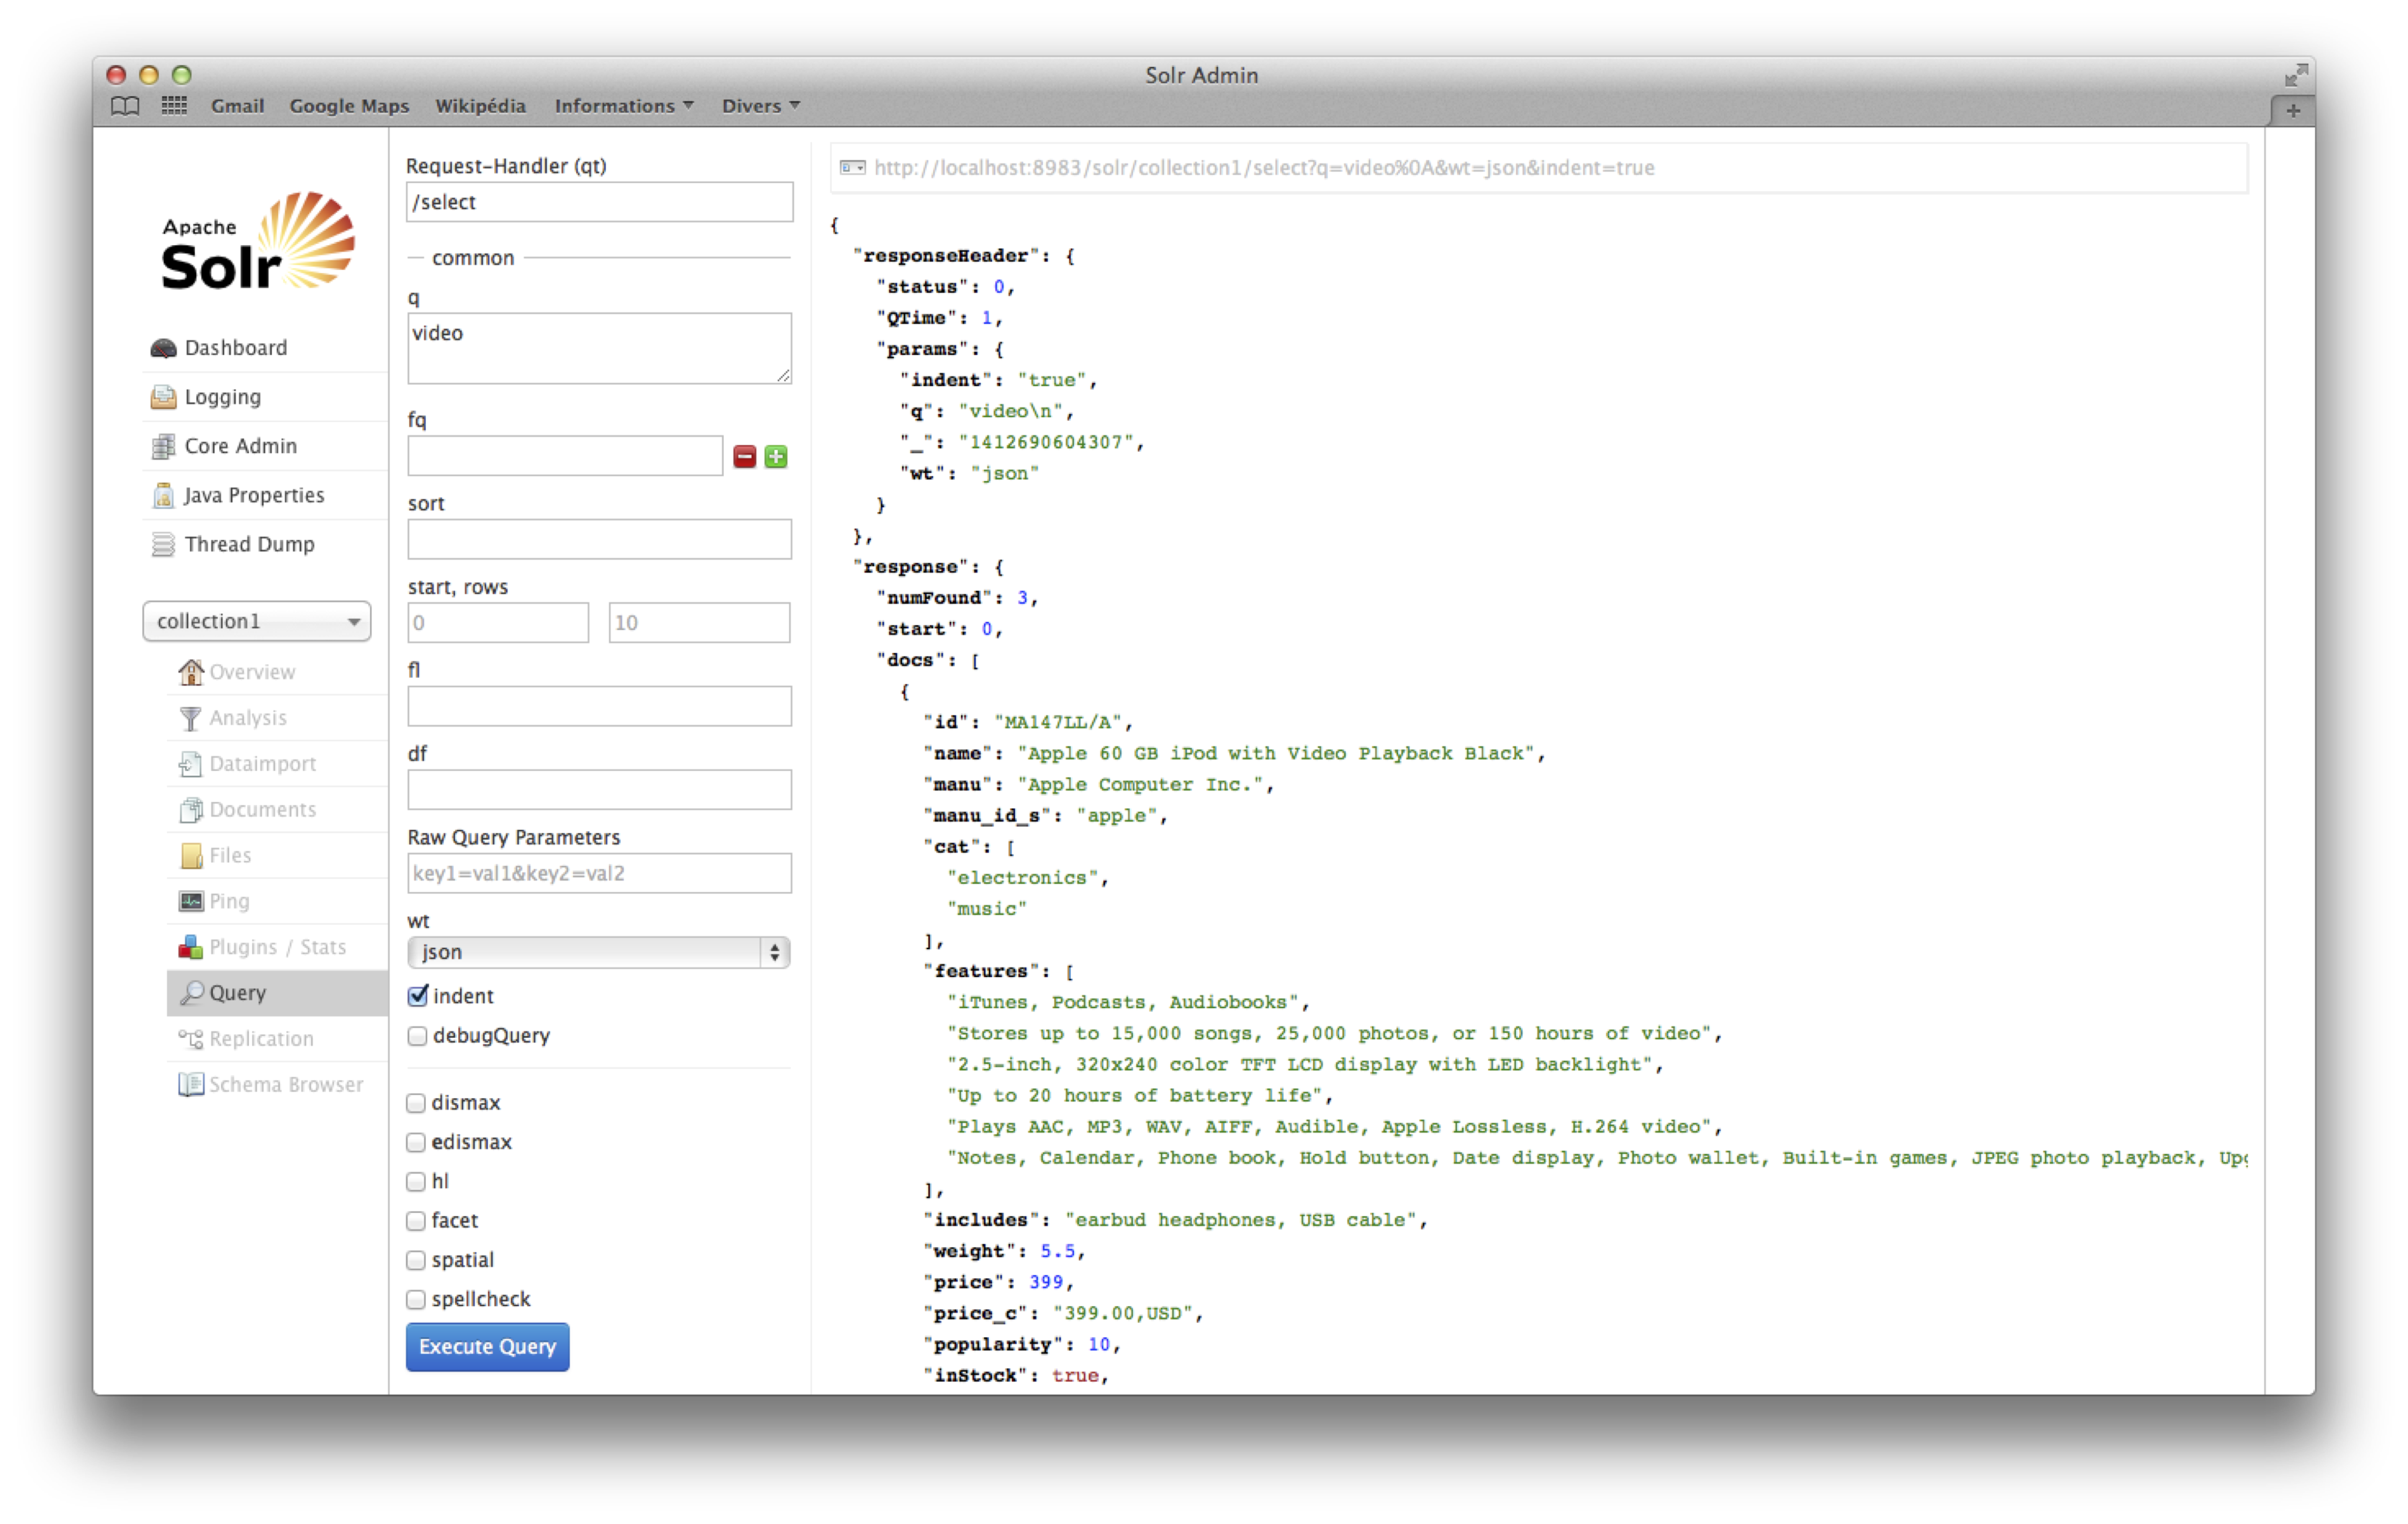
\includegraphics[width=11cm]{../figures/solr-query.png}
  \end{center}
\end{frame} % ending frame Fenêtre d'interrogation de Solr

\begin{frame}{Réponse de Solr}
  \begin{itemize}
    \item En-tête (propriétés sur l'exécution, dont temps de réponse)
    \item Liste des {\bf documents Solr} considérés comme satisfaisant les
      critères
      \begin{itemize}
        \item constitués des valeurs de champs insérés dans l'index
        \item cela ne suffira cependant souvent pas, il faudra accéder au {\bf
          document applicatif} correspondant
        \item importance du champ \variable{id} (clef d'accès base documentaire) 
      \end{itemize}
  \end{itemize}
  \caveat{Certains champs (\variable{cat} et \variable{features} par exemple) sont multivalués (ils
  sont représentés par des tableaux en JSON). L'index en a tenu compte}

\end{frame} % ending frame Réponse de Solr

%%.. important:: en fait les champs ramenés par une requête sont ceux déclarés par le schéma
   %%comme étant *stockés*. 

\begin{frame}[fragile]{Illustration de la puissance de Solr}
 \begin{itemize}
   \item recherche par mot-clef
   \item {\bf projection} (SQL) avec le paramètre \variable{fl} ({\bf field list}) :\\
\begin{minted}[frame=lines,
               baselinestretch=.9,
               fontsize=\footnotesize,
               framesep=2mm]{text}
   http://localhost:8983/solr/select?q=video&fl=id,name
\end{minted}
\item spécifier dans quel champ on cherche :\\
\begin{minted}[frame=lines,
               baselinestretch=.9,
               fontsize=\footnotesize,
               framesep=2mm]{text}
   http://localhost:8983/solr/select?q=name:black  
\end{minted}
\item pagination de résultats :\\

\begin{minted}[frame=lines,
               baselinestretch=.9,
               fontsize=\footnotesize,
               framesep=2mm]{text}
   http://localhost:8983/solr/select?q=video&start=1&rows=10
\end{minted}
\end{itemize}
\end{frame}

